\documentclass[10pt]{article}
\usepackage{amsmath,amsfonts,times}
\usepackage{graphicx,color,tikz}
\usepackage[paperwidth=17.6cm,paperheight=6.6cm,lmargin=0in,rmargin=0in,tmargin=0.in,bmargin=0.in]{geometry}
\usepackage{bm}
\usetikzlibrary{arrows.meta,calc,positioning}

% Offsets and annuli traced from their operands' level sets, drawn in a plane through the ray: a box grown into
% a box with rounded edges and corners, and a mesh's annulus as the union of its faces, each grown into a slab
% with a rounded rim (here a polyline, each segment grown into a capsule).
\definecolor{cray}{rgb}{0.10,0.35,0.80}
\definecolor{cshell}{rgb}{0.95,0.60,0.10}
\definecolor{chit}{rgb}{0.80,0.10,0.10}
\definecolor{csolid}{rgb}{0.78,0.78,0.80}

\tikzset{
  ray/.style={-{Stealth[length=2.5mm]}, line width=1.1pt, draw=cray},
  hit/.style={circle, fill=chit, draw=white, inner sep=0pt, minimum width=5pt},
  crossing/.style={circle, fill=black, inner sep=0pt, minimum width=4pt},
  capsule/.style={draw=cshell!80!black, densely dashed, thin},
  note/.style={font=\scriptsize, align=left},
  guide/.style={black!25, densely dotted},
}

\begin{document}
\nopagecolor
\centering
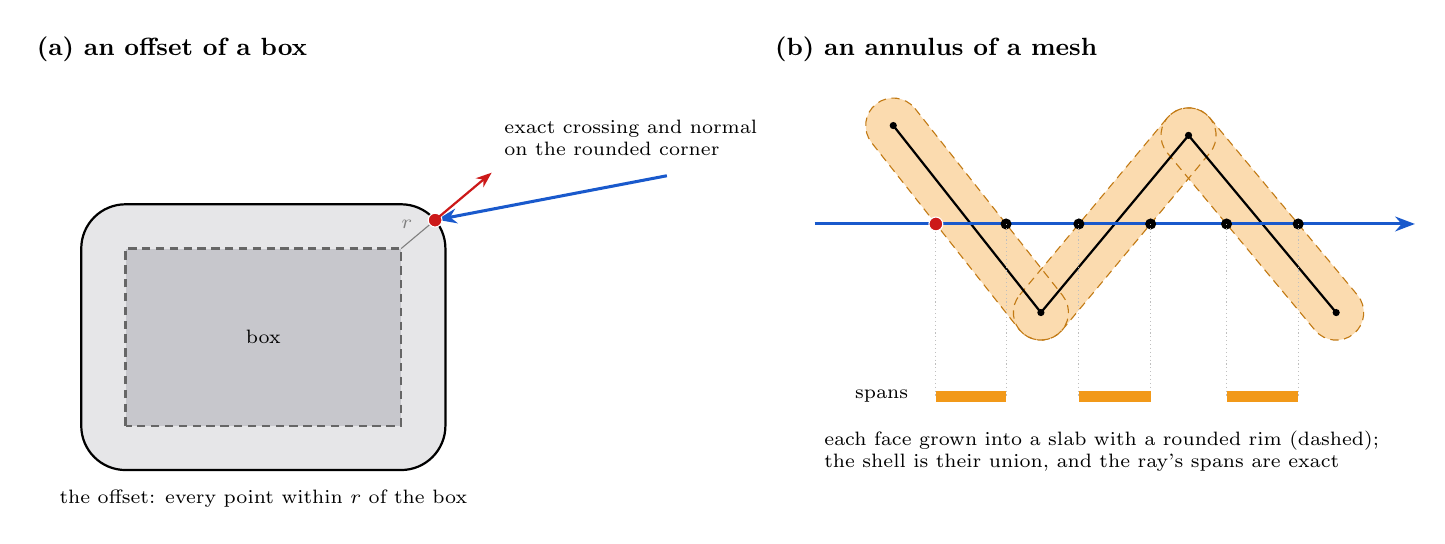
\begin{tikzpicture}[x=1.25cm, y=1.25cm]

  % ── (a) Offset of a box by r: a box with rounded edges and corners, crossed exactly.
  \begin{scope}
    \node[font=\small\bfseries, anchor=north west] at (-2.4,3.15) {(a) an offset of a box};
    \draw[thick, fill=csolid!45, rounded corners=0.5625cm] (-1.85,-1.35) rectangle (1.85,1.35);
    \draw[thick, black!60, densely dashed, fill=csolid] (-1.4,-0.9) rectangle (1.4,0.9);
    \node[font=\scriptsize] at (0,0) {box};
    \draw[black!50] (1.4,0.9) -- node[note, above left=-2pt] {$r$} (1.745,1.189);
    \draw[ray] (4.1,1.64) -- (1.765,1.193);
    \node[hit] at (1.745,1.189) {};
    \draw[chit, thick, -{Stealth[length=2mm]}] (1.745,1.189) -- ++(40:0.75);
    \node[note, anchor=south west] at (2.35,1.75) {exact crossing and normal\\on the rounded corner};
    \node[note, anchor=north] at (0,-1.45) {the offset: every point within $r$ of the box};
  \end{scope}

  % ── (b) Annulus of a mesh: the faces' slabs with rounded rims, and the spans of the ray through them.
  \begin{scope}[shift={(6.4,-0.15)}]
    \node[font=\small\bfseries, anchor=north west] at (-1.3,3.3) {(b) an annulus of a mesh};
    \draw[line width=0.7cm, line cap=round, line join=round, cshell!35] (0.0,2.3) -- (1.5,0.4) -- (3.0,2.2) -- (4.5,0.4);
    \draw[capsule] (0.22,2.474) -- (1.72,0.574) arc[start angle=38.29, delta angle=-180, radius=0.28] -- (-0.22,2.126) arc[start angle=218.29, delta angle=-180, radius=0.28] -- cycle;
    \draw[capsule] (1.285,0.579) -- (2.785,2.379) arc[start angle=140.194, delta angle=-180, radius=0.28] -- (1.715,0.221) arc[start angle=320.194, delta angle=-180, radius=0.28] -- cycle;
    \draw[capsule] (3.215,2.379) -- (4.715,0.579) arc[start angle=39.806, delta angle=-180, radius=0.28] -- (2.785,2.021) arc[start angle=219.806, delta angle=-180, radius=0.28] -- cycle;
    \draw[thick] (0.0,2.3) -- (1.5,0.4) -- (3.0,2.2) -- (4.5,0.4);
    \foreach \p in {(0.0,2.3),(1.5,0.4),(3.0,2.2),(4.5,0.4)} { \fill \p circle[radius=1.3pt]; }
    \draw[ray] (-0.8,1.3) -- (5.3,1.3);
    \foreach \x in {0.433,1.146,1.886,2.615,3.386,4.114} {
      \node[crossing] at (\x,1.3) {};
      \draw[guide] (\x,1.3) -- (\x,-0.45);
    }
    \node[hit] at (0.433,1.3) {};
    % The spans along the ray.
    \draw[line width=4pt, cshell] (0.433,-0.45) -- (1.146,-0.45);
    \draw[line width=4pt, cshell] (1.886,-0.45) -- (2.615,-0.45);
    \draw[line width=4pt, cshell] (3.386,-0.45) -- (4.114,-0.45);
    \node[note, anchor=east] at (0.25,-0.45) {spans};
    \node[note, anchor=north west] at (-0.8,-0.7) {each face grown into a slab with a rounded rim (dashed);\\the shell is their union, and the ray's spans are exact};
  \end{scope}

\end{tikzpicture}

\end{document}
